\title{Plan of Action}
\author{
		\textbf{T64PF1 \& T64NE1 } \and
        Aashish G, Athreya Chandramouli, Devesh Verma, Sachin Dev
}
\date{}

\documentclass[12pt]{article}
\usepackage{listings}
\usepackage{color}
\usepackage{xcolor}
\usepackage{textcomp}
\usepackage[pdftex]{hyperref}
\usepackage{graphicx} % for \scalebox and \raisebox macros
\newcommand\hash{\scalebox{0.8}{\raisebox{0.4ex}{\#}}}
\usepackage[section]{placeins}


\definecolor{solarized@base03}{HTML}{002B36}
\definecolor{solarized@base02}{HTML}{073642}
\definecolor{solarized@base01}{HTML}{586e75}
\definecolor{solarized@base00}{HTML}{657b83}
\definecolor{solarized@base0}{HTML}{839496}
\definecolor{solarized@base1}{HTML}{93a1a1}
\definecolor{solarized@base2}{HTML}{EEE8D5}
\definecolor{solarized@base3}{HTML}{FDF6E3}
\definecolor{solarized@yellow}{HTML}{B58900}
\definecolor{solarized@orange}{HTML}{CB4B16}
\definecolor{solarized@red}{HTML}{DC322F}
\definecolor{solarized@magenta}{HTML}{D33682}
\definecolor{solarized@violet}{HTML}{6C71C4}
\definecolor{solarized@blue}{HTML}{268BD2}
\definecolor{solarized@cyan}{HTML}{2AA198}
\definecolor{solarized@green}{HTML}{859900}
\definecolor{light-gray}{gray}{0.95}

\lstset{
  upquote=true,
  columns=fixed,
  tabsize=2,
  extendedchars=true,
  breaklines=true,
  % frame=single
  backgroundcolor=\color{light-gray},
  numbers=left,
  numbersep=5pt,
  rulesepcolor=\color{solarized@base03},
  numberstyle=\tiny\color{solarized@base01},
  basicstyle=\footnotesize\ttfamily,
  keywordstyle=\color{solarized@green},
  stringstyle=\color{solarized@cyan}\ttfamily,
  identifierstyle=\color{solarized@blue},
  commentstyle=\color{solarized@base01},
  emphstyle=\color{solarized@red}
}


\begin{document}
\maketitle


\section{Brief Summary}
The IBM Watson \emph{Natural Language Understanding} API, can be utilized to analyze features of natural langauge text. The goal of submission 1 is to build a bare-bones application which integrates the \emph{POST /analyze} functionality of the API, and utilize it to categorize some given input text. The application should be suitable for use as a boilerplate starter-project for /hub.

As of now, we've successfully managed to integrate the API's basic functionality, using the provided wrappers and have tested a few hardcoded inputs. We've drawn up wireframes and mockups for the frontend and are in the process of implementing them. Once this is completed, we can integrate it with the backend using Jinja templates. More details can be found in the next section. 

\section{Sub-Task Checklist}
\begin{itemize}
	\item{\textbf{Backend - Python-Flask/NodeJS-Express}} \hfill \textbf{Status}
		\begin{itemize}
			\item \textbf{Installation of Requirements} \hfill \textbf{Complete} \\
				To integrate the API, \emph{watson-developer-cloud} must be installed. This is done using pip (\emph{pip install --upgrade watson-developer-cloud}) for Flask and 
				npm (\emph{npm install watson-developer-cloud}) for Express.
			\item \textbf{Authentication using BlueMix Account} \hfill \textbf{Complete}\\
				In order to use the API, authentication is required. To generate the service credentials, the user has to sign up for the service using their IBM BlueMix account. 
			\item \textbf{Basic integration with Flask/Express} \hfill \textbf{Complete} \\
				Once the authentication is successful, the basic integration is done by importing the appropriate modules(\emph{NaturalLanguageUnderstandingV1}), instantiating the required class as an object(\emph{understandingObj}), and calling the appropriate methods (\emph{understandingObj.analyze()}).
			\item \textbf{Testing with Hardcoded inputs} \hfill \textbf{Complete} \\
				Given a body of text, the API returns a JSON object consisting of the category and the corresponding confidence. The integration was tested using some hardcoded bodies of text to check its functioning. An example of the input and output can be found in the next section.
			\item \textbf{Integration with Frontend} \hfill \textbf{Pending} \\
				Using Jinja templates to combine the Frontend with Flask. Similarly, integration is done with Express as well. 
		\end{itemize}
	\item{\textbf{Frontend - React-Native}}
		\begin{itemize}
			\item \textbf{Form UI} \hfill \textbf{Wireframe} \\
				TextInput tag is used for inputting the text to be passed to the API.
				The UI is minimalist with a simple Gradient style for the button.(Wireframe Uses: Gradient \hash 7956EC - \hash 2FB9F8) 
			\item \textbf{Result UI} \hfill \textbf{Wireframe} \\
				The result is shown as 3 TextViews for the 3 sets of variable. It is graphically represented using 3 ImageViews with the background colour as a Gradient (Wireframe Uses: \hash FFC066 - \hash F33573, \hash 3CECB0 - \hash 009FC5, \hash FF618C - \hash AD2AB9)
				distributed by the tag \\ \mbox{\emph{\textless JustifyContent="space-between" \textgreater}}. Currently this is a static image, but it can be modified to dynamically resize depending on the confidence value.
			\item \textbf{Error Handling} \hfill \textbf{Pending} \\
				Any obvious errors, such as invalid inputs, insufficient characters, excessive characters etc\ldots are handled at the Frontend directly.
			\item \textbf{Integration with Backend} \hfill \textbf{Pending} \\
				Using Jinja templates to combine the Frontend with Flask. Similarly, integration is done with Express as well.

		\end{itemize}
		\begin{figure}
			\centering
			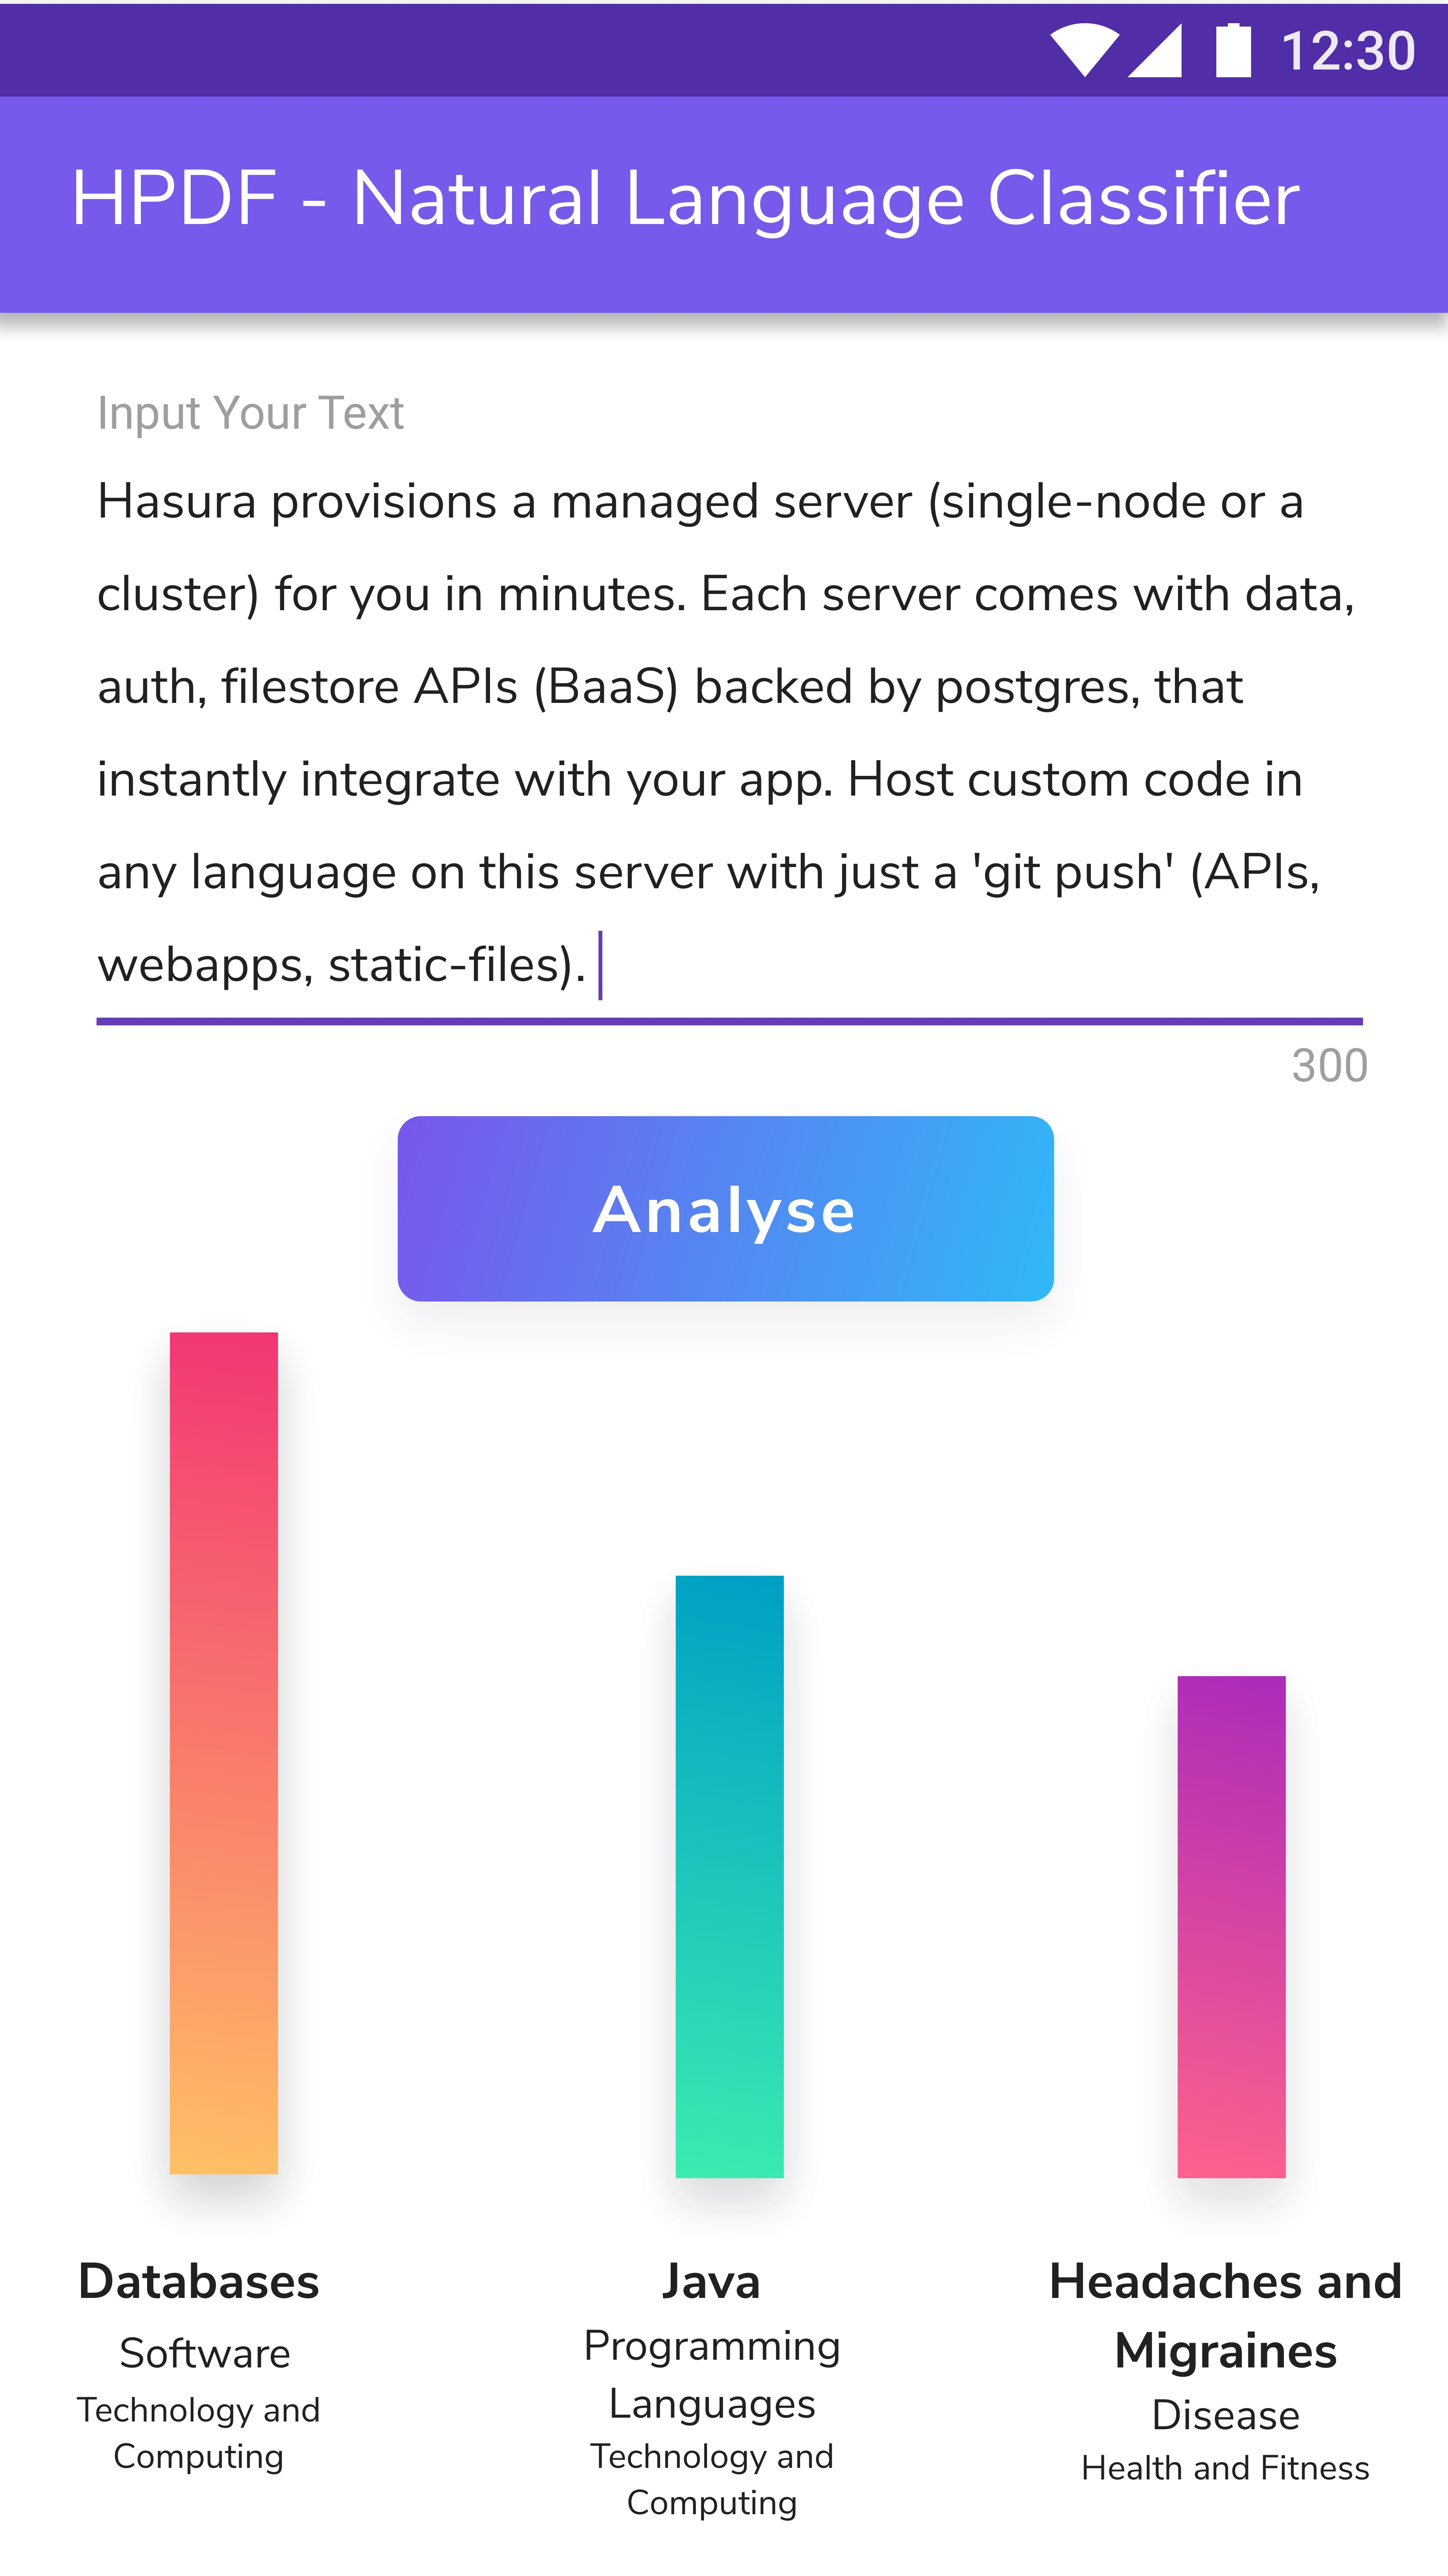
\includegraphics[width=0.6\linewidth]{wireframe.jpeg}
			\caption{Frontend Wireframe}
		\end{figure}

\end{itemize}


\section{Sample I/O}
	\underline{Input Text:}
	\begin{quote}
		"Hasura provisions a managed server (single-node or a cluster) for you in minutes.
		Each server comes with data, auth, filestore APIs (BaaS) backed by postgres, that instantly integrate with your app.
		Host custom code in any language on this server with just a 'git push' (APIs, webapps, static-files)."
	\end{quote}
	\underline{Output JSON:}\footnote{\textbf{Note}: The output is posted verbatim. This does not reflect the thoughts and views of any of the team members. We don't think Hasura is about headaches and migraines, but for some reason Watson seems to.}
	\begin{lstlisting}
{
  "categories": [
    {
      "label": "/technology and computing
      		/software/databases",
      "score": 0.436991
    },
    {
      "label": "/technology and computing
      		/programming languages/java",
      "score": 0.311278
    },
    {
      "label": "/health and fitness/disease
      		/headaches and migraines",
      "score": 0.259054
    }
  ],
  "language": "en",
  "usage": {
    "features": 1,
    "text_characters": 300,
    "text_units": 1
  }
}
	\end{lstlisting}


\section{Resources/Docs}
The Documentation for the API can be found \href{https://www.ibm.com/watson/developercloud/natural-language-understanding/api/v1/hashintroduction}{\underline {here}}. It serves as a comprehensive guide for understanding and using the API functionalities, including the \emph{POST /analyze}. The docs provide syntax (for the Node and Python wrappers), input and output format, and details about parameters and parameter types.

\section{Responsibilities}
\begin{tabular}{|l|l|l|}
\hline
\textbf{Name} & \textbf{Email} & \textbf{Allotted Framework}} \\
\hline
\hline
Aashish G & aashishgrao1@gmail.com & React-Native \\
\hline
Athreya Chandramouli & cathreya98@gmail.com & Python-Flask \\
\hline
Devesh Verma & deveshverma619@gmail.com & NodeJS-Express \\
\hline
Sachin Dev & hellosachindev@gmail.com & React-Native\\
\hline
\end{tabular}

\end{document}

